\documentclass{article}

\PassOptionsToPackage{numbers, sort&compress}{natbib}
\usepackage[final]{neurips_2019}
\usepackage[utf8]{inputenc}
\usepackage[T1]{fontenc}
\usepackage{hyperref}
\usepackage{url}
\usepackage{booktabs}
\usepackage{amsfonts}
\usepackage{amsmath}
\usepackage{amssymb}
\usepackage{nicefrac}
\usepackage{microtype}
\usepackage{graphicx}
\usepackage{xcolor}
\usepackage{multirow}
\usepackage{array}

\graphicspath{{figures/}}
\setlength{\tabcolsep}{3.2pt}
\renewcommand{\arraystretch}{1.02}
\setlength{\textfloatsep}{7pt plus 1pt minus 2pt}
\setlength{\floatsep}{5pt plus 1pt minus 1pt}
\setlength{\intextsep}{5pt plus 1pt minus 1pt}
\setlength{\abovecaptionskip}{3pt}
\setlength{\belowcaptionskip}{1pt}
\setcounter{topnumber}{4}
\setcounter{bottomnumber}{3}
\setcounter{totalnumber}{6}
\renewcommand{\topfraction}{0.92}
\renewcommand{\bottomfraction}{0.80}
\renewcommand{\textfraction}{0.07}
\renewcommand{\floatpagefraction}{0.85}

\makeatletter
\renewcommand{\@notice}{}
\makeatother

\title{Efficient Inference and Compression for Language Models:\\
Weight Compression, Attention Memory, and Speculative Distillation}

\author{%
  Muhammad Umair \\
  Lahore University of Management Sciences \\
  \texttt{25280013@lums.edu.pk}
}

\begin{document}
\maketitle

\begin{abstract}
We empirically evaluate three pillars of efficient language model inference on a single NVIDIA L4 GPU under pinned seeds, datasets, and Hugging Face revisions.
\textbf{First (Model Compression)}, across 18 post-training conditions on \texttt{Qwen2.5-1.5B}, activation-aware methods dominate naive baselines: at 50\% sparsity, Wanda cuts WikiText-2 perplexity from 127.80 (Magnitude) to 25.50 and lifts HellaSwag normalized accuracy by +18.15\,pp, while at 4-bit (4.16 effective bits/weight), AWQ achieves 17.56 perplexity and 68.20\% HellaSwag---outperforming 50\% pruning at less than half its packed storage. Dev-selected non-uniform block pruning (\texttt{ShortGPT-BI}) rescues 75\% sparsity from collapse (428.5 vs.\ 63,325 perplexity), and Taylor-weighted mixed-precision MILP (\texttt{Q3}) improves INT3 HellaSwag (+1.40\,pp raw). Yet dense FP16 execution keeps GPU latency and VRAM flat despite $2.7\times$--$3.1\times$ packed storage savings.
\textbf{Second (Efficient Attention \& KV Memory)}, IO-aware SDPA (FlashAttention) reduces FP16 attention memory by $42.8\times$ and runs $146\times$ faster than dense attention at $L=8192$, whereas pure-Python tiling is $3{,}408\times$ slower. On matched-parameter MQAR (436,736 params, 42 runs), sliding-window attention hits its exact $2(W-1)=126$ receptive-field cliff, linear attention exhibits seed-dependent stalls at $K\in\{8,16\}$, and content-based top-$k$ ($k=64$) achieves 100.0\% recall across all seeds. On 180 long-context retrieval prompts (\texttt{Qwen2.5-1.5B-Instruct}) at a matched INT4 KV budget, per-token INT4 quantization collapses to 0.0\% due to Qwen2.5 key-channel outliers, whereas KIVI (per-channel $K$, per-token $V$) retains 100.0\% and a hybrid FP16/INT2 policy reaches 99.4\% under budget---though pure-PyTorch bit-unpacking slows single-batch decoding by $6.2\times$.
\textbf{Third (Policy Distillation \& Speculative Decoding)}, LoRA distillation ($r=8$, 40k tokens) of \texttt{Qwen2.5-0.5B-Instruct} toward \texttt{Qwen2.5-1.5B-Instruct} lowers common-prefix KL and raises live $\gamma=2$ acceptance by +1.98 to +2.75\,pp (cutting target passes to 0.39/token), with on-policy distillation costing $4.66\times$ longer than off-policy (1,942\,s vs.\ 417\,s) while preserving +5.0--6.7\,pp more standalone GSM8K accuracy. Crucially, eager batch-1 latency is kernel-launch bound ($c=t_{\text{draft}}/t_{\text{target}}=0.83$), pushing break-even acceptance to $\alpha^*\approx 94\%$ and making speculative decoding slower than target-only (27.1 vs.\ 33.3\,tok/s) with no finite amortization break-even.
Code, scripts, configurations, and machine-readable results: \url{https://github.com/umairs5/atml-pa4}.
\end{abstract}

\section{Introduction and Shared Experimental Protocol}
\label{sec:intro}
Modern large language model (LLM) deployment is governed by three coupled bottlenecks: weight-memory footprint and bandwidth during decoding, quadratic attention and linear KV-cache growth over long contexts, and sequential per-token latency in autoregressive generation. Although algorithmic approximations---weight pruning and quantization, sparse or linear attention, KV compression, and distilled speculative decoding---promise substantial theoretical savings, their real-world value hinges on two questions: \emph{which structural assumptions survive realistic outlier geometries and long-range retrieval}, and \emph{when serialized or asymptotic reductions actually translate into wall-clock speedups on commodity GPUs}.

\paragraph{Unified Protocol and Cross-Cutting Theme.}
All GPU experiments run on a single NVIDIA L4 (Ada Lovelace, \texttt{sm\_89}, 24\,GiB VRAM) using Python 3.13.16, PyTorch 2.14.1+cu130 \citep{paszke2019pytorch}, \texttt{transformers==4.57.1} \citep{wolf2020transformers}, PEFT \citep{mangrulkar2022peft}, common base seed 6304, and locked dataset/model commits (Appendix~\ref{app:setup}). Throughout all three tasks, we enforce strict accounting discipline: we distinguish percentage points (pp) from relative percentages, serialized/packed bytes from allocated GPU VRAM, and analytical speedups ($\hat{S}_\gamma$) from measured wall-clock throughput ($S_\gamma$). All statistical comparisons use 2,000-resample paired bootstraps \citep{efron1993bootstrap} over aligned windows or prompts, and all hyperparameter/candidate selections in Task~1 occur strictly on a held-out C4 dev split. A unifying finding emerges across all three tasks: \emph{algorithmic compression and kernel fusion are inseparable}---without fused sparse, dequantizing, or CUDA-graphed kernels, unfused PyTorch execution routinely erases $3\times$--$6\times$ serialized savings and turns theoretical speedups into net slowdowns.

% =============================================================================
\section{Task 1: Post-Training Model Compression (Pruning and Quantization)}
\label{sec:task1}

\paragraph{Setup and Exact Accounting.}
We evaluate 18 conditions on the base \texttt{Qwen/Qwen2.5-1.5B} \citep{qwen2025qwen25} model in FP16: unpruned baseline, uniform Magnitude pruning (P1; \citealp{han2015learning}) and Wanda (P2; \citealp{sun2024wanda}) at 25/50/75\% sparsity plus 2:4 semi-structured Wanda at 50\%, dev-selected non-uniform pruning (P3) at 50/75\%, uniform group-128 asymmetric RTN quantization (Q1) and AWQ (Q2; \citealp{lin2024awq}) at INT8/4/3, and dev-selected mixed-precision quantization (Q3) at exact Q2 INT4/3 byte budgets. Exact tensor accounting verifies 28 decoder layers with 196 eligible linear matrices containing 1,310,195,712 eligible weights (2,620.4\,MB FP16) and 233,518,592 uncompressed weights (233,373,696 embeddings, 87,552 norms, 57,344 biases; 467.0\,MB FP16). Because \texttt{embed\_tokens} and \texttt{lm\_head} are tied (1 duplicate tensor of 233,373,696 weights counted once), the model has 1,543,714,304 unique parameters (3,087,428,608 FP16 bytes = 2,944.40\,MiB). Calibration uses 128 locked C4 sequences ($L=2048$; \citealp{raffel2020c4}); evaluation measures WikiText-2 \citep{merity2017wikitext} and C4 validation perplexity (50,000 tokens each, 437/177 windows), HellaSwag \citep{zellers2019hellaswag} (\texttt{acc} and length-normalized \texttt{acc\_norm} on 2,000 primary prompts for key conditions and the first 512 diagnostic prompts for all 18), and dense-FP16 inference timing (prefill 512/2048, decode 64) plus peak VRAM.

\begin{table}[t]
\centering
\scriptsize
\caption{Task 1 compression matrix on \texttt{Qwen2.5-1.5B} (NVIDIA L4, FP16 dense execution). Packed MiB includes uncompressed tensors, 1-bit sparse masks or group-128 scales/zeros, and AWQ channel scales (0.08\,MiB). HS-2k (\texttt{acc\_norm}, $n=2000$) is reported for primary conditions alongside HS-512 ($n=512$, all 18). $\Delta_{\text{cum}}$ is final-block cumulative relative $L_2$ calibration drift. Full prefill-2048 timings and raw \texttt{acc} appear in Appendix~\ref{app:task1}.}
\label{tab:task1}
\resizebox{\textwidth}{!}{%
\begin{tabular}{@{}lrrrrrrrrrr@{}}
\toprule
Condition & WT2 PPL & C4 PPL & HS-2k & HS-512 & Eff.\ b/w & Packed & Comp.\,s & $\Delta_{\text{cum}}$ & Dec-64 & VRAM \\
 & ($\Delta$) & ($\Delta$) & norm & norm & (elig.) & (MiB) & (L4) & ($L_2$) & (ms) & (MiB) \\
\midrule
FP16 Baseline & 16.11 (+0.00) & 14.96 (+0.00) & 69.40 & 58.20 & 17.00 & 2944.4 & 0.0 & --- & 1891 & 4155.0 \\
\midrule
P1 Mag 25\% & 21.33 (+5.22) & 17.99 (+3.02) & --- & 58.79 & 13.00 & 2475.8 & 0.4 & 0.390 & 1910 & 4155.5 \\
P1 Mag 50\% & 127.80 (+111.7) & 102.46 (+87.50) & 39.90 & 41.41 & 9.00 & 1851.1 & 0.4 & 0.746 & 1914 & 4155.5 \\
P1 Mag 75\% & 1.57M (+1.57M) & 1.22M (+1.22M) & --- & 28.52 & 5.00 & 1226.3 & 0.4 & 1.125 & 1915 & 4155.5 \\
P2 Wanda 25\% & 16.55 (+0.45) & 15.39 (+0.43) & --- & 59.38 & 13.00 & 2475.8 & 0.4 & 0.093 & 1916 & 4155.5 \\
P2 Wanda 50\% & 25.50 (+9.39) & 21.22 (+6.26) & 58.05 & 53.91 & 9.00 & 1851.1 & 0.4 & 0.299 & 1918 & 4155.5 \\
P2 Wanda 75\% & 63.3k (+63.3k) & 51.6k (+51.6k) & --- & 29.69 & 5.00 & 1226.3 & 0.5 & 1.006 & 1902 & 4155.5 \\
P2 Wanda 2:4 (50\%) & 67.96 (+51.86) & 51.43 (+36.47) & --- & 44.34 & 9.00 & 1851.1 & 1.4 & 0.553 & 1910 & 4155.5 \\
P3 ShortGPT-BI 50\% & \textbf{24.86} (+8.75) & \textbf{20.75} (+5.79) & 57.55 & 52.73 & 9.00 & 1851.1 & 0.4 & 0.291 & 1903 & 4155.5 \\
P3 ShortGPT-BI 75\% & \textbf{428.5} (+412.4) & \textbf{268.2} (+253.3) & --- & \textbf{32.81} & 5.00 & 1226.3 & 0.4 & 0.643 & 1912 & 4155.5 \\
\midrule
Q1 RTN INT8 & 16.08 ($-$0.02) & 14.97 (+0.01) & --- & 58.20 & 8.19 & 1724.2 & 0.7 & 0.017 & 1909 & 4155.5 \\
Q1 RTN INT4 & 18.90 (+2.79) & 16.73 (+1.77) & 67.00 & 57.81 & 4.16 & 1094.6 & 0.9 & 0.234 & 1880 & 4155.5 \\
Q1 RTN INT3 & 40.54 (+24.43) & 30.57 (+15.61) & 56.15 & 50.78 & 3.15 & 937.1 & 2.7 & 0.547 & 1893 & 4155.5 \\
Q2 AWQ INT8 & 16.11 (+0.01) & 14.97 (+0.00) & --- & 58.01 & 8.19 & 1724.3 & 162.3 & 0.009 & 1969 & 4155.6 \\
Q2 AWQ INT4 & 17.56 (+1.45) & 15.94 (+0.98) & \textbf{68.20} & \textbf{58.98} & 4.16 & 1094.6 & 164.6 & 0.142 & 1990 & 4155.6 \\
Q2 AWQ INT3 & \textbf{26.38} (+10.27) & 21.29 (+6.33) & 61.10 & 52.54 & 3.15 & 937.2 & 185.3 & 0.322 & 2002 & 4155.6 \\
Q3 Mixed INT4 & \textbf{17.54} (+1.44) & \textbf{15.92} (+0.96) & 67.80 & 58.40 & 4.16 & 1094.6 & 164.9 & 0.141 & 2020 & 4155.6 \\
Q3 Mixed INT3 & 26.58 (+10.47) & \textbf{21.28} (+6.32) & \textbf{61.90} & \textbf{53.12} & 3.15 & 937.2 & 185.9 & 0.324 & 1939 & 4155.6 \\
\bottomrule
\end{tabular}%
}
\end{table}

\paragraph{Activation awareness dominates both pruning and quantization, and low-bit quantization Pareto-dominates pruning (Table~\ref{tab:task1}, Fig.~\ref{fig:task1}a).}
We expected weighting compression error by input-activation magnitudes to preserve high-variance outlier channels \citep{sun2024wanda,lin2024awq}. The gains are decisive and statistically confirmed by paired bootstrap 95\% CIs: at 50\% sparsity, Wanda outperforms Magnitude by $-102.30$ WT2 PPL ($[-112.89, -93.72]$), $-81.23$ C4 PPL ($[-90.42, -72.86]$), and $+18.15$\,pp on HS-2k \texttt{acc\_norm} ($[+16.05, +20.25]$). Enforcing 2:4 semi-structured sparsity on Wanda at 50\% costs $+42.47$ WT2 PPL ($[+38.59, +46.83]$) and $-9.57$\,pp on HS-512 ($[-13.09, -6.05]$), quantifying the steep representational price of hardware-friendly 2-of-4 block constraints. In quantization, INT8 is effectively lossless for both Q1 and Q2 ($\Delta\text{PPL}\le 0.01$). At INT4, AWQ beats RTN by $-1.34$ WT2 PPL ($[-1.60, -1.13]$), $-0.79$ C4 PPL ($[-0.94, -0.66]$), and $+1.20$\,pp HS-2k ($[+0.15, +2.30]$); at INT3, AWQ's advantage widens to $-14.16$ WT2 PPL ($[-15.51, -13.02]$) and $+4.95$\,pp HS-2k ($[+3.30, +6.55]$). Comparing modalities at equal or smaller packed footprints, INT4 AWQ (4.16\,b/w, 1,094.6\,MiB, 17.56 PPL, 68.20\% HS-2k) soundly beats 50\% Wanda (9.00\,b/w, 1,851.1\,MiB, 25.50 PPL, 58.05\% HS-2k), and even INT3 AWQ (3.15\,b/w, 937.2\,MiB) exceeds 50\% Wanda on HellaSwag by +3.05\,pp while using half the storage.

\begin{figure}[t]
\centering
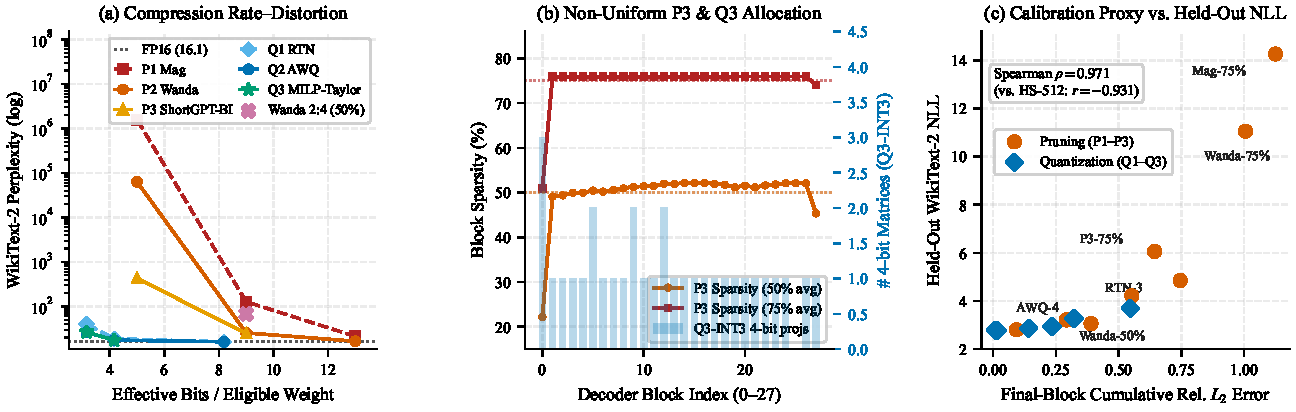
\includegraphics[width=\linewidth]{fig1_task1_compression.pdf}
\caption{Task 1 compression analysis on \texttt{Qwen2.5-1.5B}. (a) Quantization Pareto-dominates pruning across effective bit budgets. (b) Dev-selected P3 (\texttt{ShortGPT-BI}) sharply protects blocks 0 and 27, while Q3 (\texttt{MILP-Taylor}) upgrades attention projections (\texttt{v\_proj}/\texttt{k\_proj}/\texttt{o\_proj}) to 4-bit at INT3 budget. (c) Final-block cumulative calibration drift strongly tracks held-out NLL ($\rho=0.971$).}
\label{fig:task1}
\end{figure}

\paragraph{Dev-selected non-uniform allocation rescues 75\% pruning collapse and nudges INT3 downstream accuracy (Fig.~\ref{fig:task1}b, Appendix~\ref{app:task1}).}
We screened 8 non-uniform pruning candidates (OWL block/projection \citep{yin2024owl}, ShortGPT Block Influence \citep{men2024shortgpt}, and local/Fisher/Taylor marginal Wanda) strictly on C4 dev at both 50\% and 75\% sparsity. Interestingly, projection-level marginal allocators (\texttt{marginal\_local\_wanda} 29.39 dev PPL, \texttt{marginal\_taylor\_wanda} 26.55) over-pruned sensitive matrices up to 85\% and underperformed uniform Wanda (17.07) at 50\%, whereas \texttt{shortgpt\_bi\_lam0.15} achieved strong 50\% dev PPL (16.84) and crushed every rival at 75\% (236.8 vs.\ 677.9--10,411.8 dev PPL; Fig.~\ref{fig:A1}a) by sharply protecting block~0 (BI = 0.965, sparsity reduced to 22.2\% at 50\% avg / 50.9\% at 75\% avg) and block~27 (BI = 0.246, 45.4\% / 74.1\%). On held-out tests, P3 beats uniform Wanda at 50\% by $-0.64$ WT2 PPL ($[-0.76, -0.51]$) and $-0.48$ C4 PPL ($[-0.69, -0.33]$) with a slight $-0.50$\,pp HS-2k difference ($[-1.25, +0.20]$, inconclusive), and rescues 75\% sparsity by $-62{,}896$ WT2 PPL ($[-68{,}931, -57{,}284]$) and $+3.13$\,pp HS-512 ($[-1.37, +7.42]$). For Q3, we solved an exact integer program over $\{2,3,4,8\}$-bit assignments matching Q2's byte budget across 4 sensitivity objectives; unweighted MSE failed catastrophically at INT3 (55.48 dev PPL), whereas \texttt{milp\_taylor} won at both INT4 (13.12 dev PPL; bit histogram $\{3{:}2, 4{:}191, 8{:}3\}$, promoting layers 0/11/15 \texttt{v\_proj} to 8-bit) and INT3 (16.89 dev PPL; $\{2{:}3, 3{:}161, 4{:}32\}$, upgrading 25 \texttt{v\_proj}, 4 \texttt{k\_proj}, and 3 \texttt{o\_proj} matrices to 4-bit while downgrading only 3 matrices to 2-bit; Fig.~\ref{fig:A1}c). Held-out perplexity differences between Q3 and Q2 are tiny and cross zero (INT4 WT2 $-0.011$ $[-0.059, +0.033]$; INT3 $+0.205$ $[-0.045, +0.457]$), but Q3 yields a statistically significant $+1.40$\,pp raw HS-2k gain at INT3 ($[+0.50, +2.25]$, \texttt{acc\_norm} $+0.80$\,pp $[-0.30, +1.95]$).

\paragraph{Calibration drift predicts held-out NLL, while unfused execution exposes a stark storage-vs-runtime gap (Fig.~\ref{fig:task1}c).}
Full-precision AWQ rescaling equivalence passes within relative $L_2$ error $1.07\times 10^{-3}$ (0.11\%). Across all 17 compressed models, final-block cumulative calibration error $\Delta_{\text{cum}}$ correlates tightly with held-out WT2/C4 NLL (Spearman $\rho=0.971$, Pearson $r=0.879$) and HS-512 ($r=-0.931$). Note an informative diagnostic nuance: our isolated per-projection probe reported $\infty$ on AWQ layers 1--2 \texttt{down\_proj} because AWQ folds $s^{-1}$ into \texttt{up\_proj} and $s$ into \texttt{down\_proj}; evaluating \texttt{down\_proj} alone against unrescaled FP16 inputs breaks scale cancellation, whereas the end-to-end block probe restores cancellation cleanly ($\Delta_{\text{cum}}=0.142$ for AWQ-4 vs.\ $0.234$ for RTN-4). On systems efficiency, although INT3 Q2/Q3 shrinks packed storage $3.14\times$ (2,944 $\to$ 937\,MiB), dense FP16 execution leaves prefill-512 (45.3--48.4\,ms), prefill-2048 (177.4--185.7\,ms), and peak VRAM (4,155.0--4,155.6\,MiB) completely unchanged; worse, Q2/Q3 decode-64 latency \emph{increases} by 48--129\,ms (1,891 $\to$ 1,939--2,020\,ms) because \texttt{o\_proj}'s non-absorbable AWQ channel scales execute via a Python forward pre-hook. Qualitative HellaSwag inspection (Appendix~\ref{app:qual}) confirms how compression alters length-normalized margins: on \emph{Playing polo} (row 112), Wanda, P3, and Q3-INT3 recover the correct continuation that Magnitude-50\% and AWQ-INT3 lose, whereas on \emph{Removing ice from car} (row 86), aggressive pruning flips an FP16 error into a correct answer by flattening overconfident distractor log-likelihoods.

% =============================================================================
\section{Task 2: Efficient Attention Mechanisms and KV-Cache Memory}
\label{sec:task2}

\subsection{Part A: Exact IO-Aware Attention vs.\ Dense and Pure-Python Tiling}
\paragraph{Numerical verification and backend dispatch.}
We compare dense causal attention, our pure-PyTorch online-softmax tiled attention ($B_q=B_{kv}=64$; \citealp{milakov2018online,dao2022flashattention}), and \texttt{F.scaled\_dot\_product\_attention} (SDPA) for $B=2, H=4, d_h=64$ across $L\in\{256,\dots,8192\}$ in FP16 and FP32. Correctness tests pass with zero causality leakage (prefix max abs diff $= 0.0$), finite stability under extreme logits (max abs diff $1.49\times 10^{-4}$), finite all-masked handling ($0.0$), and tile-size invariance at $L=512$ across $32{\times}32$, $64{\times}64$, $128{\times}128$, and $64{\times}128$ ($\le 5.07\times 10^{-7}$ FP32; $\le 2.61\times 10^{-3}$ FP16). Probing SDPA on NVIDIA L4 (\texttt{sm\_89}) shows that FP16 supports all four backends and dispatches \texttt{FLASH\_ATTENTION} \citep{dao2024flashattention2}, whereas FP32 rejects Flash and cuDNN (\texttt{RuntimeError: No available kernel}) and falls back to \texttt{EFFICIENT\_ATTENTION}.

\begin{table}[t]
\centering
\scriptsize
\caption{Task 2 Part A scaling on NVIDIA L4 ($B=2, H=4, d_h=64$, 10 repeats). Errors are max absolute deviation vs.\ FP32 dense reference. Full 6-length ($L=256\dots 8192$) and gradient tables appear in Appendix~\ref{app:task2}.}
\label{tab:task2a}
\begin{tabular}{@{}clrrrrrr@{}}
\toprule
$L$ & Operator & \multicolumn{3}{c}{FP16 (SDPA: \texttt{FLASH})} & \multicolumn{3}{c}{FP32 (SDPA: \texttt{EFFICIENT})} \\
\cmidrule(lr){3-5}\cmidrule(lr){6-8}
 & & Out Err & Fwd+Bwd (ms) & Mem (MiB) & Out Err & Fwd+Bwd (ms) & Mem (MiB) \\
\midrule
256 & Dense & $2.02{\times}10^{-3}$ & 2.12 & 38.9 & 0.0 & 2.20 & 39.4 \\
 & Tiled-64 (Py) & $2.02{\times}10^{-3}$ & 19.20 & 31.0 & $4.77{\times}10^{-7}$ & 17.37 & 30.8 \\
 & SDPA & $2.02{\times}10^{-3}$ & \textbf{0.50} & \textbf{26.5} & $1.43{\times}10^{-6}$ & \textbf{0.60} & \textbf{27.8} \\
\midrule
1024 & Dense & $2.18{\times}10^{-3}$ & 6.75 & 276.4 & 0.0 & 7.50 & 278.4 \\
 & Tiled-64 (Py) & $1.53{\times}10^{-3}$ & 241.96 & 124.5 & $4.77{\times}10^{-7}$ & 214.79 & 112.9 \\
 & SDPA & $1.36{\times}10^{-3}$ & \textbf{0.62} & \textbf{57.3} & $1.91{\times}10^{-6}$ & \textbf{0.93} & \textbf{62.3} \\
\midrule
4096 & Dense & $1.97{\times}10^{-3}$ & 153.82 & 3,768.8 & 0.0 & 153.11 & 3,776.8 \\
 & Tiled-64 (Py) & $1.89{\times}10^{-3}$ & 3,580.24 & 1,242.2 & $7.45{\times}10^{-7}$ & 3,294.91 & 1,002.7 \\
 & SDPA & $1.43{\times}10^{-3}$ & \textbf{1.17} & \textbf{180.5} & $1.43{\times}10^{-6}$ & \textbf{9.61} & \textbf{200.6} \\
\midrule
8192 & Dense & $1.55{\times}10^{-3}$ & 611.87 & 14,753.3 & 0.0 & 606.99 & 14,769.3 \\
 & Tiled-64 (Py) & $1.53{\times}10^{-3}$ & 14,289.21 & 4,577.1 & $5.96{\times}10^{-7}$ & 13,254.01 & 3,585.5 \\
 & SDPA & $1.75{\times}10^{-3}$ & \textbf{4.19} & \textbf{344.8} & $2.50{\times}10^{-6}$ & \textbf{37.56} & \textbf{385.0} \\
\bottomrule
\end{tabular}
\end{table}

\paragraph{Tiling alone saves forward memory, but kernel fusion is what unlocks speed and backward memory (Table~\ref{tab:task2a}, Fig.~\ref{fig:task2}a).}
At $L=8192$ FP16, dense attention materializes the full $L{\times}L$ score matrix, consuming 11,553\,MiB in forward and 14,753\,MiB in forward+backward. Pure-PyTorch online tiling eliminates the forward $L^2$ matrix (264.6\,MiB forward, matching SDPA's 256.5\,MiB), but without FlashAttention's fused recomputation kernel, PyTorch autograd caches per-tile intermediates across the backward graph (4,577\,MiB vs.\ SDPA's 344.8\,MiB---a $42.8\times$ reduction vs.\ dense) and launches $O((L/64)^2)$ HBM-bound kernels, running in 14,289\,ms versus 611.9\,ms for dense and \textbf{4.19\,ms} for SDPA ($146\times$ faster than dense; $3{,}408\times$ faster than Python tiling). Thus, algorithmic tiling explains the $O(L)$ memory bound, while SRAM fusion explains the throughput gain.

\subsection{Part B: Multi-Query Associative Recall (MQAR) Under Matched Parameters}
\paragraph{Setup.}
Following Zoology \citep{arora2024zoology}, we train a 2-layer causal Transformer ($T=256, d=128, H=4, d_h=32$) across 5 attention mechanisms with \textbf{exact 0.0\% parameter delta (436,736 trainable parameters each)}: Dense (B1), Sliding Window $W=64$ (B1), Linear ELU+1 \citep{katharopoulos2020transformers} (B2), Local+Dilated \citep{beltagy2020longformer} (B2), and content-based Top-$k$ ($k=64$, B3) across associative loads $K\in\{4,8,16\}$, near/mixed training regimes, and 3 seeds (6304--6306; 42 runs total).

\begin{figure}[t]
\centering
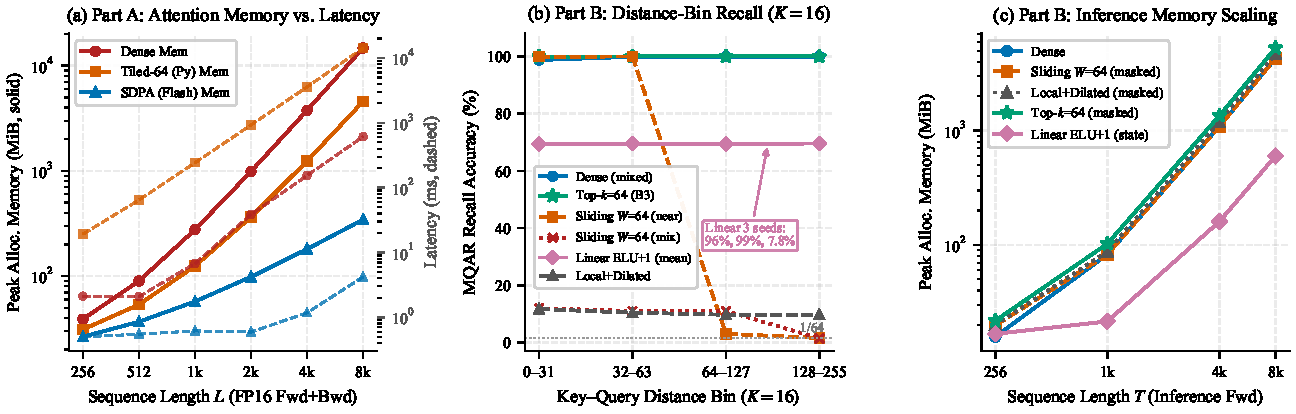
\includegraphics[width=\linewidth]{fig2_task2_ab.pdf}
\caption{Task 2 Parts A and B. (a) Part A FP16 forward+backward memory (solid) and latency (dashed): Flash SDPA achieves $O(L)$ memory and $146\times$ speedup over dense at $L=8192$. (b) Part B MQAR $K=16$ accuracy across key--query distance bins: \texttt{topk\_64} matches dense at 100\%, \texttt{sliding\_w64} drops sharply to chance beyond distance 64, and \texttt{linear\_elu1} suffers seed stalls. (c) Part B inference memory: only \texttt{linear\_elu1} avoids $O(T^2)$ mask materialization in eager PyTorch.}
\label{fig:task2}
\end{figure}

\begin{table}[t]
\centering
\scriptsize
\caption{Task 2 Part B MQAR test recall accuracy (\%, mean $\pm$ std over 3 seeds; 436,736 params for every model). Chance is $1/64 = 1.56\%$ (full vocab) and $1/K$ (in-sequence values). \texttt{W64 Ctrl} evaluates dense models under a test-time $W=64$ mask.}
\label{tab:task2b}
\resizebox{\textwidth}{!}{%
\begin{tabular}{@{}llcccccc@{}}
\toprule
Group / Mechanism & Train ($K$, Reg.) & Near (\%) & Far (\%) & Mixed (\%) & Dist.\ $[64,128)$ & Dist.\ $[128,256)$ & W64 Ctrl (N / F) \\
\midrule
B1 Dense & $K{=}4$, mixed & 100.0 $\pm$ 0.0 & 100.0 $\pm$ 0.0 & 100.0 $\pm$ 0.0 & 50.3 & 52.4 & 100.0 / 1.46 \\
B1 Dense & $K{=}8$, mixed & 100.0 $\pm$ 0.0 & 100.0 $\pm$ 0.0 & 100.0 $\pm$ 0.0 & 72.2 & 73.3 & 100.0 / 1.63 \\
B1 Dense & $K{=}16$, mixed & 99.8 $\pm$ 0.3 & 99.9 $\pm$ 0.1 & 99.9 $\pm$ 0.1 & 99.9 & 99.9 & 99.9 / 1.57 \\
B1 Dense & $K{=}16$, near & 100.0 $\pm$ 0.0 & 99.7 $\pm$ 0.2 & 99.8 $\pm$ 0.2 & 100.0 & 99.7 & 100.0 / 1.50 \\
\midrule
B1 Sliding $W{=}64$ & $K{=}4$, near & 100.0 $\pm$ 0.0 & 1.46 $\pm$ 0.1 & 26.0 $\pm$ 0.2 & 2.66 & 1.59 & --- \\
B1 Sliding $W{=}64$ & $K{=}16$, near & 100.0 $\pm$ 0.0 & 1.58 $\pm$ 0.1 & 22.4 $\pm$ 0.1 & 3.07 & 1.60 & --- \\
B1 Sliding $W{=}64$ & $K{=}16$, mixed & 7.04 $\pm$ 0.1 & 1.42 $\pm$ 0.1 & 4.25 $\pm$ 0.3 & 11.1 & 1.46 & --- \\
\midrule
B2 Linear ELU+1 & $K{=}4$, mixed & 99.2 $\pm$ 0.4 & 99.2 $\pm$ 0.4 & 99.3 $\pm$ 0.3 & 44.9 & 47.3 & --- \\
B2 Linear ELU+1 & $K{=}8$, mixed & 70.5 $\pm$ 49.9 & 70.3 $\pm$ 50.3 & 70.4 $\pm$ 50.2 & 51.6 & 52.5 & --- \\
B2 Linear ELU+1 & $K{=}16$, mixed & 67.7 $\pm$ 51.9 & 67.7 $\pm$ 52.4 & 67.7 $\pm$ 52.4 & 69.4 & 69.6 & --- \\
B2 Local+Dilated & $K{=}4$, mixed & 31.0 $\pm$ 4.4 & 29.2 $\pm$ 1.9 & 29.6 $\pm$ 3.1 & 11.7 & 12.6 & --- \\
B2 Local+Dilated & $K{=}16$, mixed & 6.57 $\pm$ 0.1 & 6.19 $\pm$ 0.1 & 6.15 $\pm$ 0.1 & 9.72 & 9.73 & --- \\
\midrule
\textbf{B3 Top-$k$=64} & $K{=}16$, mixed & \textbf{100.0 $\pm$ 0.0} & \textbf{100.0 $\pm$ 0.0} & \textbf{100.0 $\pm$ 0.0} & \textbf{100.0} & \textbf{100.0} & --- \\
\bottomrule
\end{tabular}%
}
\end{table}

\paragraph{Content-addressable routing, not attended token count, determines long-range associative recall (Table~\ref{tab:task2b}, Fig.~\ref{fig:task2}b--c).}
Dense attention solves MQAR at every load (99.8--100.0\%) and even generalizes zero-shot from near-only training at $K=16$ to 99.7\% far recall; applying a test-time $W=64$ mask drops its far recall straight to 1.50--1.63\% ($\approx 1/64$ chance), confirming genuine long-range retrieval. By contrast, \texttt{sliding\_w64} trained on near queries achieves 100.0\% near recall but collapses to 1.58\% on far queries (exact cliff past its 2-layer receptive field $2(W-1)=126$), and fails even on near queries (7.04\%) when trained on mixed data because unrecoverable far-query gradients destabilize optimization. \texttt{local\_dilated} struggles at $K=4$ (31.0\%) and sits at the $1/K=6.25\%$ in-sequence value-guessing floor at $K=16$ (6.57\%) because fixed strided gaps miss arbitrary key positions. \texttt{linear\_elu1} (recurrent state $= 16.5$\,KB/layer vs.\ 256\,KB dense KV at $T=256$) reaches 99.2\% at $K=4$ but exhibits sharp seed-level phase-transition instability under higher load: at $K=8$, seeds reach 99.4\%, \textbf{12.9\%}, and 99.4\%; at $K=16$, seeds reach 96.0\%, 99.3\%, and \textbf{7.8\%} (Fig.~\ref{fig:A2}a). Crucially, \textbf{B3 \texttt{topk\_64}}---which attends to the exact same 64-position budget as \texttt{sliding\_w64} (57,472 attended pairs/layer) with zero extra parameters---achieves \textbf{100.0\% $\pm$ 0.0\%} across near, far, and mixed on all three seeds (and converges faster than dense!). Yet the inference sweep (Fig.~\ref{fig:task2}c, Appendix~\ref{app:task2}) underscores our systems theme: only \texttt{linear\_elu1} avoids $O(T^2)$ score materialization in PyTorch (600\,MiB vs.\ 4,297\,MiB dense at $T=8192$, running faster at 160.8 vs.\ 194.7\,ms), whereas dense-masked \texttt{topk\_64} still computes all $T^2$ scores to select top-64 (5,288\,MiB, 395.6\,ms at $T=8192$), requiring approximate index structures or fused sparse kernels for wall-clock gains.

\subsection{Part C: KV-Cache Compression at Matched INT4 Budget on \texttt{Qwen2.5-1.5B-Instruct}}
\paragraph{Setup, Length Audit, and Equivalence Check.}
We evaluate 6 KV-cache policies on 180 long-context code-retrieval prompts (2 nominal lengths $\times$ 3 evidence positions $\times$ 3 distractor counts $\{0,2,8\} \times 10$ cases) on \texttt{Qwen2.5-1.5B-Instruct}. Our token-length audit shows nominal 2048 prompts average $L_{\text{ctx}}=2{,}626.7$ context tokens ($[2604,2648]$) + $L_q=34.7$ query tokens, and nominal 4096 prompts average $L_{\text{ctx}}=5{,}215.9$ ($[5192,5242]$) + $34.7$ query tokens, with 26--27 evidence tokens. All compressed policies are matched to the exact serialized INT4 KIVI budget $M_4(L)$ ($\approx 28.7\%$ of FP16 context KV bytes). C1 split-prefill equivalence passes on 18/18 stratified prompts (all finite, 18/18 top-1 match, max abs logit diff $0.090$--$0.250$, mean $0.007$--$0.009$).

\begin{table}[t]
\centering
\scriptsize
\caption{Task 2 Part C KV-cache compression on \texttt{Qwen2.5-1.5B-Instruct} ($n=180$ prompts) at matched INT4 KIVI budget $M_4(L)$. Because \texttt{full\_fp16} scores 100.0\% (180/180), unconditional and conditional-on-FP16 accuracies are identical. Evid.\ Ret.\ is mean fraction of evidence-span KV tokens kept in FP16.}
\label{tab:task2c}
\resizebox{\textwidth}{!}{%
\begin{tabular}{@{}lrrrrrrrrr@{}}
\toprule
Policy & Exact & Answer & Post-Prefill & Evid. & Ctx Packed & FP16 & Comp. & Decode & Peak \\
 & Match (\%) & NLL & KL vs.\ FP16 & Ret. & (MiB) & Frac. & (ms) & (ms) & (MiB) \\
\midrule
\texttt{full\_fp16} & 100.0 & 0.0010 & 0.0000 & 1.000 & 107.22 & 1.000 & 2.9 & 191.0 & 4355 \\
\texttt{evict\_sink\_recent} & 33.3 & 1.8375 & 2.1138 & 0.333 & 30.71 & 0.287 & 4.0 & 190.2 & 4257 \\
\texttt{evict\_question\_aware} & 98.9 & 0.0071 & 0.0006 & 0.935 & 30.71 & 0.287 & 87.8 & 187.5 & 5013 \\
\texttt{quant\_int4\_tok} & \textbf{0.0} & 4.4286 & 5.6705 & 1.000 & 30.71 & 0.287 & 33.7 & 547.3 & 4387 \\
\textbf{\texttt{quant\_int4\_kivi}} & \textbf{100.0} & \textbf{0.0016} & 0.0023 & 1.000 & 30.71 & 0.287 & 34.7 & 206.7 & 4387 \\
\textbf{\texttt{hybrid\_fp16\_int2}} & \textbf{99.4} & 0.0064 & 0.0038 & 0.869 & \textbf{29.64} & \textbf{0.275} & 174.6 & 187.7 & 5013 \\
\bottomrule
\end{tabular}%
}
\end{table}

\begin{figure}[t]
\centering
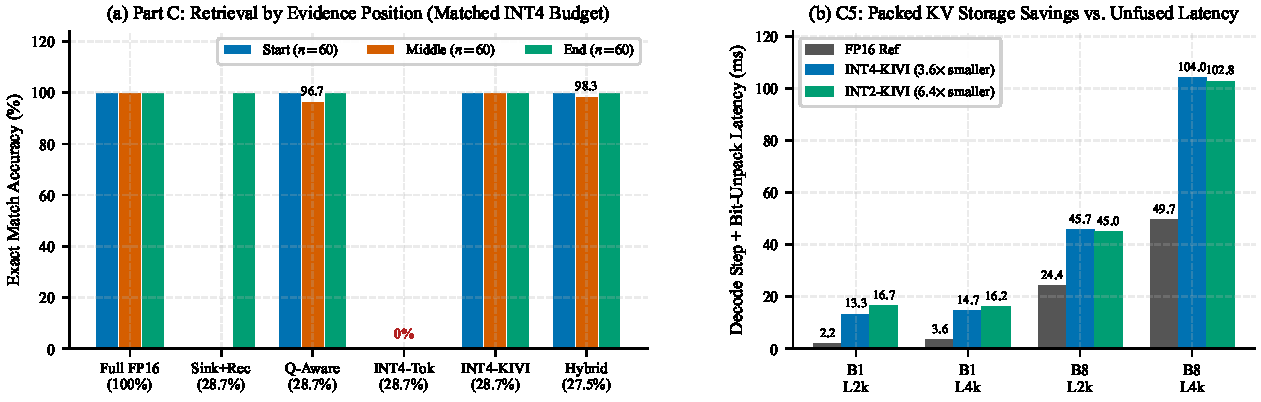
\includegraphics[width=\linewidth]{fig3_task2_c_kv.pdf}
\caption{Task 2 Part C KV-cache compression. (a) Matched-budget retrieval by evidence position: \texttt{evict\_sink\_recent} fails whenever evidence leaves the recent window, \texttt{quant\_int4\_tok} collapses to 0\%, while \texttt{quant\_int4\_kivi} (100\%) and \texttt{hybrid\_fp16\_int2} (99.4\%) recover full accuracy. (b) C5 real bit-packed benchmark: $3.6\times$--$6.4\times$ storage savings incur a $2.1\times$--$6.2\times$ unfused bit-unpacking latency penalty.}
\label{fig:task2c}
\end{figure}

\paragraph{Key-channel geometry makes quantization axis critical; question-aware eviction and KIVI/hybrid policies preserve retrieval (Table~\ref{tab:task2c}, Fig.~\ref{fig:task2c}a).}
At the matched 28.7\% budget, \texttt{evict\_sink\_recent} \citep{xiao2024streamingllm} achieves 100.0\% on \texttt{end} evidence (60/60) but 0.0\% on \texttt{start} and \texttt{middle} (0/120), yielding 33.3\% overall. Scoring context tokens via query attention (\texttt{evict\_question\_aware}; inspired by \citealp{zhang2023h2o,li2024snapkv}) lifts evidence retention from 33.3\% to 93.5\% and exact match to \textbf{98.9\%} (178/180; paired bootstrap $+65.6$\,pp $[+58.9, +72.2]$), missing only 2 prompts with middle evidence and 8 distractors (e.g., predicting \texttt{66265} instead of \texttt{66263} on \texttt{KV-2048-middle-8-09}; Appendix~\ref{app:qual}). Most strikingly, \textbf{per-token INT4 quantization (\texttt{quant\_int4\_tok}) collapses completely to 0.0\% (0/180)}, driving post-prefill KL to 5.67 and generating repetitive gibberish (\texttt{"airport river river..."}). Why? \texttt{Qwen2.5} has large learned attention projection biases (\texttt{k\_proj.bias}) creating persistent channel-wise key outliers; per-token min--max scaling stretches the 16-level grid across outlier channels and destroys low-variance signal channels. Simply transposing keys to per-channel quantization (\textbf{\texttt{quant\_int4\_kivi}}; \citealp{liu2024kivi}) restores \textbf{100.0\% (180/180; $+100.0$\,pp over per-token INT4)}, with NLL $0.0016$ vs.\ $0.0010$ for FP16 (paired $\Delta\text{NLL}=+0.0006$ $[+0.0004, +0.0009]$). Our \textbf{\texttt{hybrid\_fp16\_int2}} policy (question-aware FP16 retention + INT2 KIVI tail) stays strictly below budget (29.64\,MiB = 27.5\% FP16) and achieves \textbf{99.4\% (179/180)}, beating \texttt{evict\_question\_aware} by $+0.56$\,pp ($[-1.11, +2.78]$) and missing only a single 8-distractor middle prompt (\texttt{KV-2048-middle-8-05}, predicting \texttt{48210} vs.\ \texttt{48823} when only 65.5\% of the evidence span stayed in FP16).

\paragraph{C5 real bit-packing exposes an unfused dequantization bottleneck (Fig.~\ref{fig:task2c}b, Appendix~\ref{app:task2}).}
Benchmarking real bit-packed KIVI tensors across $B\in\{1,8\}$ and $L\in\{2048,4096\}$ confirms exact byte-formula agreement: at $B=8, L=4096$, serialized KV drops from 939.5\,MB (FP16) to 264.2\,MB (INT4-KIVI, $3.56\times$ smaller) and 146.8\,MB (INT2-KIVI, $6.40\times$ smaller). However, pure-PyTorch bit-unpacking into FP16 before SDPA adds 10.1--53.5\,ms per decode step: at $B=1, L=2048$, decode latency jumps from 2.16\,ms (FP16) to 13.33\,ms (INT4-KIVI, $6.17\times$ slower) and peak allocated VRAM \emph{doubles} (156.1 vs.\ 77.7\,MB) while holding both packed and unpacked buffers; at $B=8, L=4096$, decode slows from 49.68\,ms to 104.02\,ms ($2.09\times$). Fused quantized-KV attention kernels are thus essential to convert serialized KV compression into serving speedups.

% =============================================================================
\section{Task 3: Policy Distillation and Speculative Decoding}
\label{sec:task3}

\paragraph{Step 1 Exactness Validation and Distillation Cost Accounting.}
We pair target \texttt{Qwen2.5-1.5B-Instruct} with draft \texttt{Qwen2.5-0.5B-Instruct} (verified identical tokenizer and chat template). Step~1 lossless speculative sampling validation \citep{leviathan2023speculative,chen2023accelerating} passes every gate: on a 100,000-trial 3-symbol Markov chain ($\gamma=2$, 27 joint sequences, minimum expected count 900), our sampler yields $\chi^2=23.34$ ($p=0.6135 \ge 0.01$), whereas a broken residual negative control ($r=p$) is overwhelmingly rejected ($\chi^2=13{,}306.4, p=0.00$); self-speculative acceptance equals 1.000; and real-model KV-cache rollback preserves exact cache length with max FP16 logit diff $0.0337$. We then distill the 0.5B draft with LoRA ($r=8, \alpha=16$ on all 7 projections; 1,081,344 trainable params = 0.22\% of 495.1M total) using forward KL over exactly 40,000 teacher-scored tokens (30k GSM8K math \citep{cobbe2021gsm8k} + 10k short structured tasks) across 2 seeds (6304, 6305), comparing \textbf{off-policy} (fixed teacher rollout pool) vs.\ \textbf{on-policy} (live student rollouts scored by teacher; \citealp{zhou2024distillspec,agarwal2024gkd}). Under \texttt{transformers==4.57.1}, \texttt{model.generate()} rejects the upstream \texttt{generator=} kwarg; we fixed this via \texttt{torch.random.fork\_rng} (\texttt{generate\_prefix\_banks\_compat.py}), preserving exact seeds, prompt order, and positions (Appendix~\ref{app:setup}). Wall-clock distillation cost differs sharply (Fig.~\ref{fig:A3}a): off-policy totals \textbf{417.4\,s / 416.2\,s} (279.4\,s teacher pool prep + 30--32\,s teacher scoring + 106\,s student fwd/bwd/opt), whereas on-policy totals \textbf{1,938.1\,s / 1,946.4\,s} (\textbf{4.66$\times$ slower}), because sequential batch-1 student rollouts alone consume 1,806--1,814\,s (93\% of runtime; peak VRAM $\approx 6.1$\,GiB for both). Merging LoRA adapters takes 3.4--8.4\,s (mean abs logit diff vs.\ unmerged $0.0073$--$0.0079$) and eliminates a \textbf{+47.2\% draft latency penalty} (2,581\,ms unmerged vs.\ 1,753\,ms merged; $+34.4\%$ total latency).

\begin{figure}[t]
\centering
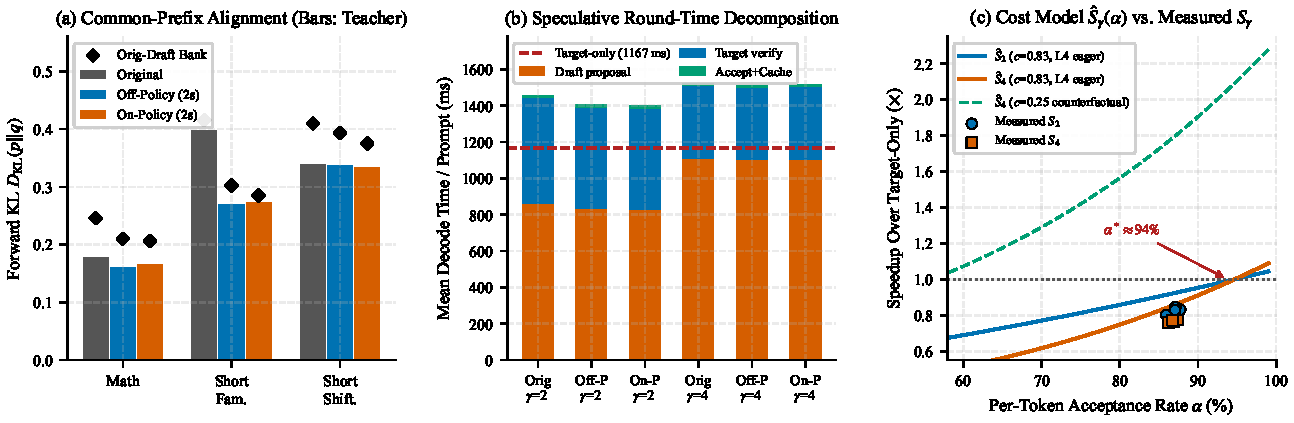
\includegraphics[width=\linewidth]{fig4_task3_speculative.pdf}
\caption{Task 3 distillation and speculative decoding on NVIDIA L4. (a) Common-prefix Forward KL drops most on \texttt{short\_familiar} across both teacher (bars) and original-draft (diamonds) prefix banks. (b) Four-part round-time breakdown: 24-layer 0.5B draft proposals dominate 28-layer 1.5B verification, exceeding target-only time (red dashed). (c) Measured $(c=0.83, v_\gamma=1.19)$ shifts break-even to $\alpha^*\approx 94\%$, whereas a $c=0.25$ counterfactual predicts $>1.8\times$ speedup.}
\label{fig:task3}
\end{figure}

\paragraph{Distillation narrows common-prefix divergence, with largest gains on familiar short tasks and subtle on-policy advantages on draft prefixes (Fig.~\ref{fig:task3}a, Fig.~\ref{fig:A3}b).}
Evaluating all 5 drafts on locked common prefix banks separates policy alignment from prefix drift. On the \texttt{teacher} bank (3,875 positions), overall Forward KL drops from 0.234 (\texttt{original}) to 0.196--0.200 (\texttt{offpolicy}) and 0.202 (\texttt{onpolicy}), raising expected single-token acceptance $1-\text{TV}$ from 85.2\% to 85.7--85.8\% (off-policy) and 85.0\% (on-policy). Gains concentrate in \texttt{short\_familiar} (Forward KL $0.400 \to 0.267$--$0.284$, $E[\text{acc}]$ $+3.3$ to $+4.0$\,pp) and early tokens $[1,16]$ ($0.224 \to 0.161$--$0.173$), while \texttt{math} is already tightly aligned ($0.180 \to 0.162$--$0.167$, $E[\text{acc}]\approx 87$--$88\%$). Crucially, on the \texttt{original\_draft} bank (3,876 positions), \texttt{onpolicy} achieves slightly lower Forward KL than \texttt{offpolicy} (0.230--0.234 vs.\ 0.237--0.242; original 0.289), confirming that training on self-generated rollouts reduces exposure bias on off-teacher prefixes, though off-policy retains a small edge in TV/expected acceptance (83.6\% vs.\ 83.3\%). Target-vs-speculative consistency is verified both offline---the \texttt{exact\_spec\_original\_gamma4} bank (3,535 positions) mirrors \texttt{teacher}-bank rankings ($E[\text{acc}]=87.9\% \to 88.1$--$88.3\%$ off-policy)---and live, where target-only and speculative runs match in EOS rate (45.4\% vs.\ 45.8\% at $\gamma=2$) and mean length (40.1 vs.\ 40.7 tokens).

\begin{table}[t]
\centering
\scriptsize
\caption{Task 3 live speculative decoding benchmark (120 prompts $\times$ 2 reps = 240 evals per row, $T=0.7$, max 64 tokens) and analytical cost model on NVIDIA L4. Target-only throughput averages 33.3\,tok/s across all matched runs. Upfront cost includes pool prep + training + merge; since $\Delta t/\text{req}<0$ (speculative is slower), amortization break-even is $\infty$ (nonexistent).}
\label{tab:task3spec}
\resizebox{\textwidth}{!}{%
\begin{tabular}{@{}lcrrrrrrrrrr@{}}
\toprule
Draft & $\gamma$ & Acc/Ex & Acc/Pr & $\mathbb{E}[\text{pref}]$ & Tgt/tok & Spec & Meas. & Pred. & $\alpha^*$ & Draft/Ver & Upfront \\
 & & (\%) & (\%) & (tok) & passes & tok/s & $S_{\text{dec}}$ & $\hat{S}_\gamma$ & (\%) & (ms / ms) & (s) \\
\midrule
\texttt{original} & 2 & 85.95 & 79.65 & 1.63 & 0.394 & 26.84 & 0.802 & 0.924 & 93.6 & 863 / 583 & 0.0 \\
\texttt{offpolicy\_s6304} & 2 & 87.48 & 81.94 & 1.67 & 0.389 & 27.07 & 0.834 & 0.939 & 93.6 & 833 / 558 & 425.8 \\
\texttt{offpolicy\_s6305} & 2 & \textbf{87.73} & \textbf{82.15} & \textbf{1.69} & \textbf{0.387} & \textbf{27.12} & 0.831 & \textbf{0.941} & 93.6 & 836 / 559 & 419.6 \\
\texttt{onpolicy\_s6304} & 2 & 87.10 & 81.44 & 1.66 & 0.390 & 26.92 & \textbf{0.845} & 0.935 & 93.6 & 822 / 551 & 1941.5 \\
\texttt{onpolicy\_s6305} & 2 & 87.08 & 81.35 & 1.66 & 0.390 & 26.91 & 0.829 & 0.935 & 93.6 & 839 / 562 & 1949.9 \\
\midrule
\texttt{original} & 4 & 86.84 & 70.07 & 2.67 & 0.276 & 25.42 & 0.763 & 0.866 & 94.1 & 1108 / 405 & 0.0 \\
\texttt{offpolicy\_s6304} & 4 & 86.73 & 70.53 & 2.73 & 0.274 & 25.48 & 0.762 & 0.864 & 94.1 & 1109 / 402 & 425.8 \\
\texttt{offpolicy\_s6305} & 4 & \textbf{87.45} & \textbf{71.96} & \textbf{2.77} & \textbf{0.270} & \textbf{25.77} & \textbf{0.773} & \textbf{0.877} & 94.1 & 1096 / 397 & 419.6 \\
\texttt{onpolicy\_s6304} & 4 & 86.22 & 69.57 & 2.67 & 0.275 & 25.26 & 0.760 & 0.856 & 94.1 & 1114 / 402 & 1941.5 \\
\texttt{onpolicy\_s6305} & 4 & 86.76 & 70.57 & 2.70 & 0.273 & 25.39 & 0.772 & 0.865 & 94.1 & 1099 / 397 & 1949.9 \\
\bottomrule
\end{tabular}%
}
\end{table}

\paragraph{Distillation significantly boosts acceptance, yet kernel-launch latency ($c=0.83$) prevents wall-clock speedup and amortization (Table~\ref{tab:task3spec}, Fig.~\ref{fig:task3}b--c).}
In live speculative decoding ($240$ evals/row), off-policy distillation raises $\gamma=2$ acceptance significantly over \texttt{original}: paired prompt-level bootstrap confirms $+1.98$\,pp ($[+0.21, +3.85]$) for \texttt{s6304} and $+2.75$\,pp ($[+1.02, +4.65]$) for \texttt{s6305} (with \texttt{short\_familiar} jumping from 78.6\% to 86.0--87.4\%), cutting target verification passes/token from 1.00 to 0.387 ($\gamma=2$) and 0.270 ($\gamma=4$). On-policy gains $+1.49$--$1.51$\,pp at $\gamma=2$ ($[-0.52, +3.59]$, CIs straddle zero) and trails off-policy by $-1.15$ to $-1.40$\,pp at $\gamma=4$ ($[-2.77, -0.11]$). \textbf{Yet every speculative configuration is slower than target-only (33.3\,tok/s $\to$ 26.8--27.1\,tok/s at $\gamma=2$, $S_{\text{dec}}=0.80$--$0.85$; 25.3--25.8\,tok/s at $\gamma=4$, $S_{\text{dec}}=0.76$--$0.77$).} Isolated step timings diagnose the exact cause: at prompt lengths 64/128/256, one 0.5B draft step takes 26.7--27.3\,ms while one 1.5B target step takes 32.1--32.7\,ms, yielding \textbf{$c = t_{\text{draft}}/t_{\text{target}} = 0.816$--$0.835$} (not $\approx 0.33$ from parameter count!), because at batch size 1 in eager PyTorch, 24 transformer layers vs.\ 28 layers is Python/CUDA kernel-launch bound rather than compute bound. Moreover, target verification of $\gamma+1$ tokens costs $v_\gamma = 1.18$--$1.20$. Under the analytical model $\hat{S}_\gamma(\alpha) = \frac{1-\alpha^{\gamma+1}}{(1-\alpha)(\gamma c + v_\gamma)}$, break-even requires $\alpha^*=93.6\%$ ($\gamma=2$) and $94.1\%$ ($\gamma=4$)---exceeding empirical acceptance (86--88\%) and predicting $\hat{S}_\gamma\in[0.86, 0.94]$. The remaining $\sim 0.10$ gap between $\hat{S}_\gamma$ and measured $S_{\text{dec}}$ arises from dual prefill, accept/residual sampling (9--10\,ms), cache updates (2.6--2.9\,ms), and early EOS truncation on short prompts: math (64 tokens) reaches $S=0.83$--$0.84$ vs.\ 0.64--0.70 on 12-token \texttt{short\_shifted}, and our 24-prompt ignore-EOS fixed-64 diagnostic (\texttt{diag24}) lifts $S_{\text{tot}}$ to $0.84$--$0.85$ (Appendix~\ref{app:task3}). Because $\Delta t/\text{req}\in[-0.39, -0.24]$\,s is negative, upfront distillation cost has \emph{no finite break-even request count} here; however, Fig.~\ref{fig:task3}c shows that in a compiled/larger-target regime with $c=0.25$ and $v_4=1.15$, break-even drops to $\alpha^*=48\%$ and our 87.5\% acceptance would yield $\hat{S}_4=1.84\times$ (amortizing 420\,s of off-policy distillation in $\sim 770$ requests).

\begin{table}[t]
\centering
\scriptsize
\caption{Task 3 standalone greedy accuracy and format compliance (\%). Math uses GSM8K (512-token cap, $n=60$; never evaluated on 64-token speed runs); short tasks use a 32-token cap ($n=30$ each). Unextractable rate is 0.0\% across all models.}
\label{tab:task3acc}
\begin{tabular}{@{}lcccccc@{}}
\toprule
Model & \multicolumn{2}{c}{GSM8K Math ($n=60$)} & \multicolumn{2}{c}{Short Familiar ($n=30$)} & \multicolumn{2}{c}{Short Shifted ($n=30$)} \\
\cmidrule(lr){2-3}\cmidrule(lr){4-5}\cmidrule(lr){6-7}
 & Acc (\%) & Trunc (\%) & Acc (\%) & Fmt (\%) & Acc (\%) & Fmt (\%) \\
\midrule
Target 1.5B & \textbf{66.7} & 5.0 & 33.3 & 33.3 & 66.7 & 66.7 \\
Original 0.5B & 48.3 & 5.0 & 33.3 & 33.3 & 76.7 & 76.7 \\
\texttt{offpolicy\_s6304} & 36.7 & 1.7 & 33.3 & 33.3 & 83.3 & 83.3 \\
\texttt{offpolicy\_s6305} & 35.0 & 5.0 & 33.3 & 33.3 & \textbf{93.3} & \textbf{93.3} \\
\texttt{onpolicy\_s6304} & 41.7 & 1.7 & 33.3 & 33.3 & 33.3 & 33.3 \\
\texttt{onpolicy\_s6305} & 41.7 & 5.0 & 33.3 & 33.3 & 90.0 & 90.0 \\
\bottomrule
\end{tabular}
\end{table}

\paragraph{Acceptance gains diverge from standalone reasoning accuracy (Table~\ref{tab:task3acc}).}
Although speculative decoding preserves the exact target distribution regardless of draft quality, standalone evaluation reveals a striking trade-off. On GSM8K (512-token cap), KL-only distillation over 40k tokens degrades standalone math accuracy from 48.3\% (\texttt{original}) to 35.0--36.7\% for off-policy, whereas on-policy retains \textbf{41.7\%} on both seeds (+5.0 to +6.7\,pp over off-policy), aligning with GKD's claim that self-generated feedback mitigates compounding multi-step reasoning errors \citep{agarwal2024gkd} (illustrated on \texttt{GSM8K-0031}; Appendix~\ref{app:qual}). On \texttt{short\_familiar}, every model---including the 1.5B target---scores identically at 33.3\%, locked 1-to-1 to exact format compliance (verbose preambles hit the 32-token cap). On \texttt{short\_shifted}, distillation strongly improves terse format compliance and accuracy from 76.7\% to 83.3--93.3\% across three runs, but exhibits seed sensitivity in \texttt{onpolicy\_s6304} (33.3\%, reverting to verbose explanations).

% =============================================================================
\section{Conclusion and Limitations}
\label{sec:conclusion}
Across model compression, attention/KV memory, and speculative decoding, two overarching lessons emerge. First, \emph{respecting activation and key-channel geometry is non-negotiable}: activation-aware Wanda/AWQ, content-addressable top-$k$ attention, and per-channel KIVI KV quantization separate near-lossless 3--4$\times$ compression from total collapse (0\% for per-token INT4 KV, 1.57M PPL for 75\% magnitude pruning). Second, \emph{algorithmic reductions do not self-compile into latency gains}: without fused sparse/low-bit matmuls (Task~1), SRAM-fused attention (Task~2A) and dequantizing KV kernels (Task~2C), or CUDA-graphed/lower-$c$ draft-target pairings (Task~3), eager PyTorch execution turns $3\times$--$6\times$ memory reductions and $2.6\times$ fewer target passes into neutral or negative wall-clock speedups.

\paragraph{Limitations.}
Our study is scoped to a single NVIDIA L4 GPU, single-seed Task~1 compression (fixed calibration set), synthetic MQAR ($T=256$) and synthetic key-retrieval KV benchmarks, and one eager 0.5B/1.5B model pair over a 40k-token distillation budget. Evaluating fused INT4/2:4 kernels (e.g., Marlin/cuSPARSELt), Triton dequantizing KV attention, and CUDA-graphed 0.5B/7B speculative pairs are natural next steps to close the algorithmic-to-systems gap quantified here.

\clearpage
\bibliographystyle{plainnat}
\bibliography{references}

% =============================================================================
\clearpage
\appendix
\section{Environment, Locked Revisions, and Compatibility Notes}
\label{app:setup}

All GPU experiments executed on a single NVIDIA L4 (24\,GiB VRAM, Ada Lovelace \texttt{sm\_89}) with Python 3.13.16, PyTorch 2.14.1+cu130, CUDA 13.0, \texttt{transformers==4.57.1}, \texttt{huggingface\_hub==0.36.2}, and PEFT. All unit test suites passed prior to full runs: Task~1 (6/6 tests in 0.37\,s), Task~2 (4/4 tests in 0.42\,s), and Task~3 (3/3 tests in 15.30\,s). Table~\ref{tab:revisions} records the exact pinned Hugging Face commit SHAs from \texttt{configs/local\_source\_revisions.json}.

\begin{table}[h]
\centering
\scriptsize
\caption{Pinned Hugging Face repository commit SHAs and core experimental hyperparameters.}
\label{tab:revisions}
\begin{tabular}{@{}lll@{}}
\toprule
Asset / Model & Repository & Pinned Commit SHA \\
\midrule
Base LLM (Task 1) & \texttt{Qwen/Qwen2.5-1.5B} & \texttt{8faed761d45a263340a0528343f099c05c9a4323} \\
Target LLM (Tasks 2C, 3) & \texttt{Qwen/Qwen2.5-1.5B-Instruct} & \texttt{989aa7980e4cf806f80c7fef2b1adb7bc71aa306} \\
Draft LLM (Task 3) & \texttt{Qwen/Qwen2.5-0.5B-Instruct} & \texttt{7ae557604adf67be50417f59c2c2f167def9a775} \\
C4 Validation & \texttt{allenai/c4} & \texttt{1588ec454efa1a09f29cd18ddd04fe05fc8653a2} \\
WikiText-2 & \texttt{Salesforce/wikitext} & \texttt{b08601e04326c79dfdd32d625aee71d232d685c3} \\
HellaSwag & \texttt{Rowan/hellaswag} & \texttt{218ec52e09a7e7462a5400043bb9a69a41d06b76} \\
GSM8K & \texttt{openai/gsm8k} & \texttt{740312add88f781978c0658806c59bc2815b9866} \\
\bottomrule
\end{tabular}
\end{table}

\paragraph{Compatibility Notes.}
(1) In \texttt{transformers==4.57.1}, \texttt{Qwen2DecoderLayer.forward} returns a bare \texttt{Tensor} rather than a 1-tuple; our Task~1 calibration and AWQ block search handle both return types.
(2) Upstream \texttt{setup\_data.py --prefix-banks} passes \texttt{generator=gen} to \texttt{model.generate()}, which raises \texttt{ValueError: model\_kwargs not used: ['generator']} under pinned \texttt{transformers==4.57.1}. We implemented \texttt{scripts/generate\_prefix\_banks\_compat.py} using \texttt{torch.random.fork\_rng} + \texttt{torch.manual\_seed} inside generation calls, reproducing exact upstream prompt ordering, seeds, temperature ($T=0.7$), and position sampling across all common and own-rollout banks.
(3) On Google Colab, pre-installed \texttt{torchao==0.10.0} conflicted with PEFT's import path and was uninstalled before Task~3 execution.

% =============================================================================
\section{Task 1 Extended Diagnostics and Dev-Selection Grids}
\label{app:task1}

Table~\ref{tab:t1_dev} reports the complete C4-dev candidate selection grids for P3 (8 candidates at 50\% and 75\% sparsity) and Q3 (4 MILP objectives at exact Q2 INT4 and INT3 byte budgets). Figure~\ref{fig:A1} visualizes the P3 75\% dev selection, Q3 MILP dev comparison, and Q3-INT3's $7\times 28$ per-projection bit allocation map. Table~\ref{tab:t1_ci} lists all 95\% paired bootstrap confidence intervals (2,000 resamples over 437 WikiText-2 windows, 177 C4 windows, and 2,000/512 HellaSwag prompts).

\begin{figure}[h]
\centering
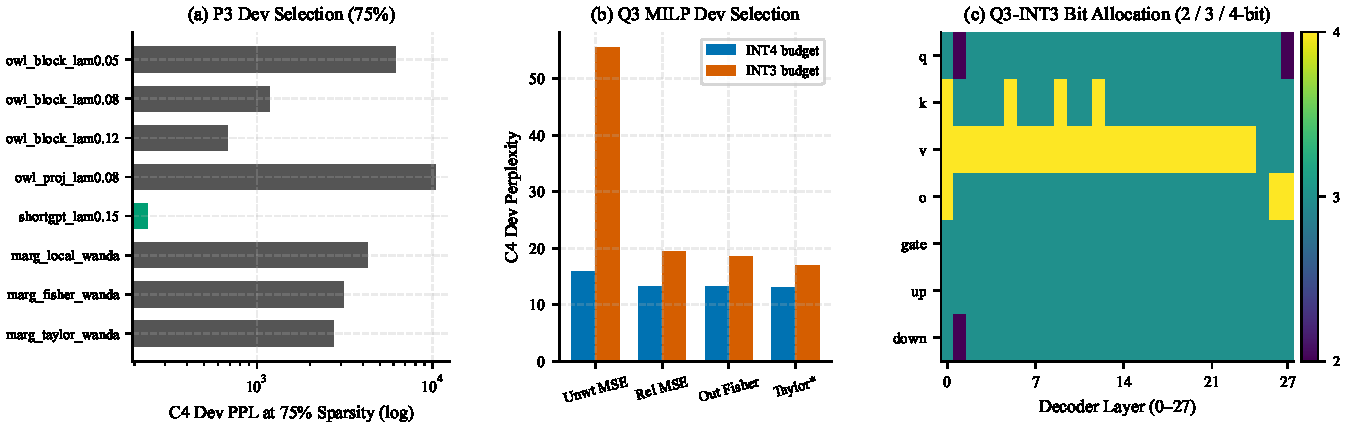
\includegraphics[width=\linewidth]{figA1_task1_dev_and_q3.pdf}
\caption{Task 1 dev-only selection and Q3 allocation map. (a) \texttt{shortgpt\_bi\_lam0.15} outperforms all 7 rival non-uniform pruning candidates by $>2.8\times$ on C4 dev at 75\% sparsity. (b) \texttt{milp\_taylor} achieves lowest C4 dev PPL at both INT4 and INT3 budgets. (c) Q3-INT3 concentrates 4-bit upgrades on \texttt{v\_proj} (layers 0--24), \texttt{k\_proj} (layers 0, 5, 9, 12), and \texttt{o\_proj} (layers 0, 26, 27).}
\label{fig:A1}
\end{figure}

\begin{table}[h]
\centering
\scriptsize
\caption{Task 1 C4-dev selection grids for P3 (8 candidates) and Q3 (4 MILP candidates). Selected methods (\texttt{shortgpt\_bi\_lam0.15} and \texttt{milp\_taylor}) are bolded.}
\label{tab:t1_dev}
\begin{tabular}{@{}llcccc@{}}
\toprule
\multicolumn{6}{c}{\textbf{P3 Non-Uniform Pruning Candidates (C4 Dev PPL; Uniform Wanda: 17.07 @ 50\%, 29,887 @ 75\%)}} \\
\midrule
Candidate & Unit & 50\% Dev PPL & 50\% Range & 75\% Dev PPL & 75\% Range \\
\midrule
\texttt{owl\_block\_lam0.05} & block & 16.83 & [0.436, 0.536] & 6,166.9 & [0.686, 0.786] \\
\texttt{owl\_block\_lam0.08} & block & 16.90 & [0.398, 0.558] & 1,180.6 & [0.648, 0.808] \\
\texttt{owl\_block\_lam0.12} & block & 17.16 & [0.346, 0.587] & 677.9 & [0.598, 0.818] \\
\texttt{owl\_proj\_lam0.08} & proj & 16.95 & [0.355, 0.515] & 10,411.8 & [0.605, 0.765] \\
\textbf{\texttt{shortgpt\_bi\_lam0.15}} & block & \textbf{16.84} & [0.222, 0.522] & \textbf{236.8} & [0.509, 0.760] \\
\texttt{marginal\_local\_wanda} & proj & 29.39 & [0.100, 0.850] & 4,249.0 & [0.150, 0.850] \\
\texttt{marginal\_fisher\_wanda} & proj & 16.37 & [0.101, 0.801] & 3,095.9 & [0.100, 0.850] \\
\texttt{marginal\_taylor\_wanda} & proj & 26.55 & [0.201, 0.850] & 2,738.9 & [0.352, 0.850] \\
\midrule
\multicolumn{6}{c}{\textbf{Q3 Mixed-Precision MILP Candidates (C4 Dev PPL; Q2 AWQ: 13.13 @ INT4, 17.01 @ INT3)}} \\
\midrule
Candidate & Objective & INT4 Dev PPL & INT4 $\{2,3,4,8\}$ & INT3 Dev PPL & INT3 $\{2,3,4,8\}$ \\
\midrule
\texttt{milp\_unweighted\_mse} & Unweighted MSE & 15.96 & $\{14, 28, 137, 17\}$ & 55.48 & $\{44, 102, 50, 0\}$ \\
\texttt{milp\_rel\_mse} & Relative MSE & 13.24 & $\{0, 7, 133, 56\}$ & 19.39 & $\{11, 75, 109, 1\}$ \\
\texttt{milp\_output\_fisher} & Output Fisher & 13.26 & $\{0, 25, 113, 58\}$ & 18.49 & $\{19, 108, 55, 14\}$ \\
\textbf{\texttt{milp\_taylor}} & First-Order Taylor & \textbf{13.12} & $\{0, 2, 191, 3\}$ & \textbf{16.89} & $\{3, 161, 32, 0\}$ \\
\bottomrule
\end{tabular}
\end{table}

\begin{table}[h]
\centering
\scriptsize
\caption{Task 1 paired bootstrap 95\% confidence intervals (2,000 resamples; A minus B). Negative $\Delta$PPL favors A; positive $\Delta$HS (pp) favors A.}
\label{tab:t1_ci}
\resizebox{\textwidth}{!}{%
\begin{tabular}{@{}lcccc@{}}
\toprule
Comparison (A vs.\ B) & WT2 $\Delta$PPL [95\% CI] & C4 $\Delta$PPL [95\% CI] & HS-2k \texttt{acc\_norm} (pp) & HS-2k raw \texttt{acc} (pp) \\
\midrule
P2 Wanda vs.\ P1 Mag (50\%) & $-102.3$ [$-112.9, -93.7$] & $-81.23$ [$-90.42, -72.86$] & $+18.15$ [$+16.05, +20.25$] & $+10.30$ [$+8.70, +12.05$] \\
Wanda 2:4 vs.\ Unstruct (50\%) & $+42.47$ [$+38.59, +46.83$] & $+30.21$ [$+26.97, +33.91$] & $-9.57^*$ [$-13.09, -6.05$] & $-5.86^*$ [$-8.59, -2.93$] \\
P3 vs.\ P2 Wanda (50\%) & $-0.64$ [$-0.76, -0.51$] & $-0.48$ [$-0.69, -0.33$] & $-0.50$ [$-1.25, +0.20$] & $-0.70$ [$-1.30, -0.15$] \\
P3 vs.\ P2 Wanda (75\%) & $-62{,}896$ [$-68{,}931, -57{,}284$] & $-51{,}360$ [$-67{,}492, -38{,}448$] & $+3.13^*$ [$-1.37, +7.42$] & $+1.17^*$ [$-1.56, +3.91$] \\
Q2 AWQ vs.\ Q1 RTN (INT4) & $-1.34$ [$-1.60, -1.13$] & $-0.79$ [$-0.94, -0.66$] & $+1.20$ [$+0.15, +2.30$] & $+0.55$ [$-0.35, +1.50$] \\
Q2 AWQ vs.\ Q1 RTN (INT3) & $-14.16$ [$-15.51, -13.02$] & $-9.28$ [$-10.54, -8.24$] & $+4.95$ [$+3.30, +6.55$] & $+3.85$ [$+2.60, +5.15$] \\
Q3 vs.\ Q2 AWQ (INT4) & $-0.011$ [$-0.059, +0.033$] & $-0.018$ [$-0.046, +0.013$] & $-0.40$ [$-0.95, +0.10$] & $+0.10$ [$-0.35, +0.55$] \\
Q3 vs.\ Q2 AWQ (INT3) & $+0.205$ [$-0.045, +0.457$] & $-0.010$ [$-0.170, +0.140$] & $+0.80$ [$-0.30, +1.95$] & $+1.40$ [$+0.50, +2.25$] \\
\bottomrule
\multicolumn{5}{l}{\footnotesize $^*$Evaluated on the 512-prompt diagnostic HellaSwag split.}
\end{tabular}%
}
\end{table}

% =============================================================================
\section{Task 2 Extended Scaling, Learning Curves, and C5 Benchmark}
\label{app:task2}

Figure~\ref{fig:A2} presents the Part~B MQAR $K=16$ learning curves (illustrating \texttt{topk\_64}'s rapid phase transition at step 1,500 vs.\ \texttt{linear\_elu1}'s delayed emergence at step 3,000 and seed 6306 stall) and Part~A numerical error stability across $L=256\dots 8192$. Table~\ref{tab:t2_c5} gives the complete C5 real bit-packed encode/decode latency and peak allocated memory benchmark across all $B\times L$ cells.

\begin{figure}[h]
\centering
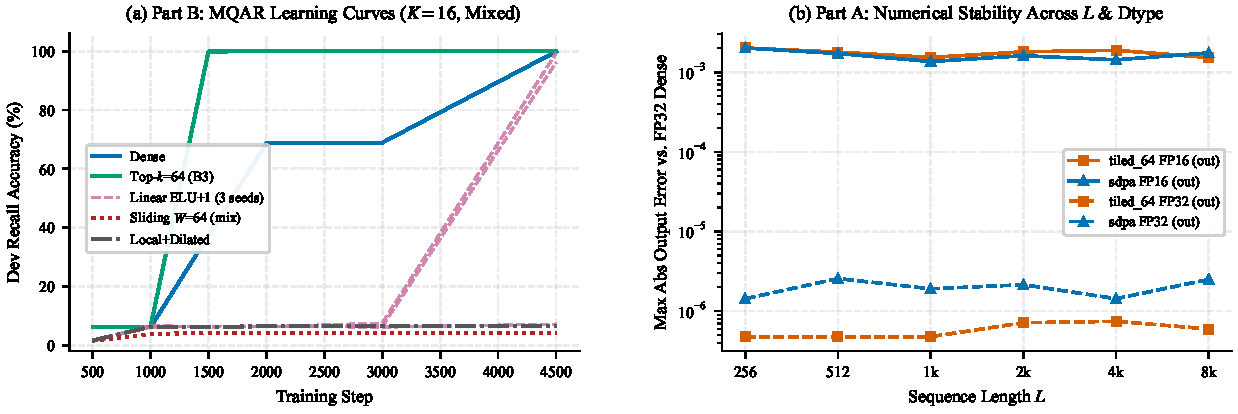
\includegraphics[width=\linewidth]{figA2_task2_mqar_curves.pdf}
\caption{Task 2 supplementary diagnostics. (a) Part~B MQAR $K=16$ dev accuracy over training steps: \texttt{topk\_64} snaps to 100\% by step 1,500 (faster than dense), while \texttt{linear\_elu1} stalls on 1/3 seeds. (b) Part~A output max absolute error remains bounded ($\le 2.5\times 10^{-6}$ FP32, $\le 2.0\times 10^{-3}$ FP16) up to $L=8192$.}
\label{fig:A2}
\end{figure}

\begin{table}[h]
\centering
\scriptsize
\caption{Task 2 Part C (C5) real bit-packed KV encode/decode benchmark on NVIDIA L4 (28 layers, 2 KV heads, $d_h=128$, 10 repeats). Serialized bytes exactly match theoretical formulas for all formats.}
\label{tab:t2_c5}
\begin{tabular}{@{}ccrrrrrrr@{}}
\toprule
$B$ & $L$ & Format & Serialized & Compression & Pack & Unpack & Decode+Unpack & Peak Alloc. \\
 & & & (MB) & vs.\ FP16 & (ms) & (ms) & (ms) & (MB) \\
\midrule
1 & 2048 & FP16 Ref & 58.72 & $1.00\times$ & --- & --- & 2.16 & 77.68 \\
1 & 2048 & INT4-KIVI & 16.52 & $3.56\times$ & 17.89 & 10.17 & 13.33 & 156.13 \\
1 & 2048 & INT2-KIVI & 9.18 & $6.40\times$ & 21.13 & 12.94 & 16.68 & 148.79 \\
\midrule
1 & 4096 & FP16 Ref & 117.44 & $1.00\times$ & --- & --- & 3.65 & 155.28 \\
1 & 4096 & INT4-KIVI & 33.03 & $3.56\times$ & 18.14 & 10.09 & 14.66 & 312.17 \\
1 & 4096 & INT2-KIVI & 18.35 & $6.40\times$ & 21.26 & 12.83 & 16.19 & 297.49 \\
\midrule
8 & 2048 & FP16 Ref & 469.76 & $1.00\times$ & --- & --- & 24.42 & 621.47 \\
8 & 2048 & INT4-KIVI & 132.12 & $3.56\times$ & 25.00 & 21.51 & 45.68 & 1,249.04 \\
8 & 2048 & INT2-KIVI & 73.40 & $6.40\times$ & 25.83 & 20.06 & 45.03 & 1,190.32 \\
\midrule
8 & 4096 & FP16 Ref & 939.52 & $1.00\times$ & --- & --- & 49.68 & 1,242.25 \\
8 & 4096 & INT4-KIVI & 264.24 & $3.56\times$ & 73.42 & 53.46 & 104.02 & 2,497.37 \\
8 & 4096 & INT2-KIVI & 146.80 & $6.40\times$ & 74.15 & 51.88 & 102.83 & 2,379.93 \\
\bottomrule
\end{tabular}
\end{table}

% =============================================================================
\section{Task 3 Extended Distillation, Workload Breakdown, and Ignore-EOS Diagnostics}
\label{app:task3}

Figure~\ref{fig:A3} shows the wall-clock distillation cost breakdown (off-policy 416--417\,s vs.\ on-policy 1,938--1,946\,s, dominated by 1,806--1,814\,s of sequential student rollouts) and token-position-bin alignment curves across $[1,16]$, $[17,32]$, $[33,64]$, and $[65,192]$. Table~\ref{tab:t3_sub} details the workload-level breakdown of live speculative decoding (\texttt{spec120}) and the 24-prompt ignore-EOS fixed-64 diagnostic (\texttt{diag24}), confirming that short early-EOS prompts incur proportionally larger prefill and round-boundary overhead ($S=0.64$--$0.70$ on 12-token \texttt{short\_shifted} vs.\ $0.84$--$0.85$ on fixed-64 \texttt{diag24}).

\begin{figure}[h]
\centering
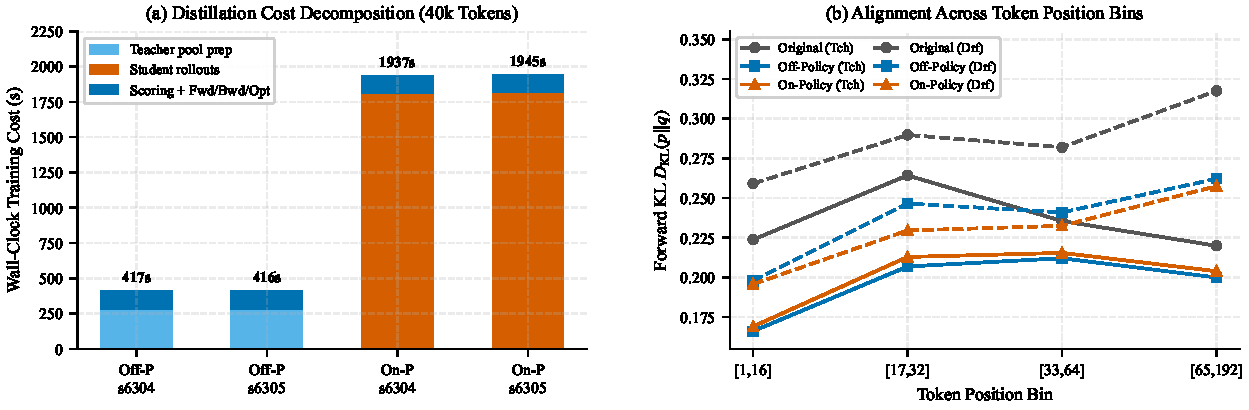
\includegraphics[width=\linewidth]{figA3_task3_distill_and_pos.pdf}
\caption{Task 3 distillation cost and positional alignment. (a) On-policy student rollouts account for 93\% of on-policy runtime ($4.66\times$ slower than off-policy). (b) Forward KL reductions peak in early positions $[1,16]$ and hold across both teacher and draft-induced prefixes.}
\label{fig:A3}
\end{figure}

\begin{table}[h]
\centering
\scriptsize
\caption{Task 3 workload breakdown ($\gamma=2$) on \texttt{spec120} and fixed-64 ignore-EOS diagnostic (\texttt{diag24}, $n=24$).}
\label{tab:t3_sub}
\begin{tabular}{@{}lcccccccc@{}}
\toprule
Draft ($\gamma=2$) & \multicolumn{2}{c}{Math ($\bar{L}=64$)} & \multicolumn{2}{c}{Short Fam.\ ($\bar{L}\approx 20$)} & \multicolumn{2}{c}{Short Shift.\ ($\bar{L}\approx 12$)} & \multicolumn{2}{c}{\texttt{diag24} Fixed-64} \\
\cmidrule(lr){2-3}\cmidrule(lr){4-5}\cmidrule(lr){6-7}\cmidrule(lr){8-9}
 & Acc/Ex & $S_{\text{tot}}$ & Acc/Ex & $S_{\text{tot}}$ & Acc/Ex & $S_{\text{tot}}$ & Spec tok/s & $S_{\text{tot}}$ \\
\midrule
\texttt{original} & 87.6\% & 0.834 & 78.6\% & 0.723 & 83.4\% & 0.696 & 27.13 & 0.843 \\
\texttt{offpolicy\_s6304} & 88.3\% & 0.837 & 87.4\% & 0.763 & 79.4\% & 0.668 & 27.79 & 0.851 \\
\texttt{offpolicy\_s6305} & 88.8\% & 0.841 & 86.0\% & 0.758 & 79.1\% & 0.657 & 27.68 & 0.846 \\
\texttt{onpolicy\_s6304} & 87.8\% & 0.833 & 87.4\% & 0.757 & 78.2\% & 0.638 & 27.54 & 0.845 \\
\texttt{onpolicy\_s6305} & 87.7\% & 0.831 & 87.3\% & 0.773 & 79.6\% & 0.659 & 27.14 & 0.837 \\
\bottomrule
\end{tabular}
\end{table}

% =============================================================================
\section{Verbatim Qualitative Case Studies}
\label{app:qual}

\paragraph{Task 1 (HellaSwag Compression Cases).}
\begin{itemize}\setlength{\itemsep}{2pt}
\item \textbf{Pruning Recovery (Row 112, \emph{Playing polo}):} Context: \emph{``A group of men on donkeys play a form of polo on a dirt field. The''} Gold (0): \emph{``camera pans to people watching the game.''} FP16 selects (0) (\texttt{norm\_ll} $-0.629$ vs.\ distractor (2) $-0.865$). \texttt{P1 Mag 50\%} collapses margin and picks (2) (\emph{``men fall to the ground.''}, $-1.007$ vs.\ $-1.008$), whereas \texttt{P2 Wanda 50\%} ($-0.787$), \texttt{P3 50\%} ($-0.779$), and \texttt{Q3 Mixed INT3} ($-0.715$ vs.\ $-0.736$) recover (0) while \texttt{Q2 AWQ INT3} still fails ($-0.811$ vs.\ $-0.796$).
\item \textbf{Quantization Recovery (Row 320, \emph{Having an ice cream}):} Context: \emph{``A child sitting at restaurant table places his hands in a dessert... The adult''} Gold (3): \emph{``keeps the child from spilling the food on the floor and helps feed him.''} All 50\% pruning methods fail (picking (2)), and \texttt{Q2 AWQ INT3} fails (picking (1), $-0.572$ vs.\ $-0.615$), whereas all INT4 methods and \texttt{Q3 Mixed INT3} ($-0.634$ vs.\ $-0.658$) preserve gold (3).
\item \textbf{Unexpected Flip (Row 86, \emph{Removing ice from car}):} FP16 erroneously prefers (0) (\emph{``finishes and turns off the wipers.''}, $-0.463$) over gold (1) (\emph{``opens the doors on his car and gets in.''}, $-0.510$). Interestingly, \texttt{P1/P2/P3 50\%} and \texttt{Q1 INT4} flip to gold (1) because pruning penalizes the lexical repetition ``wipers'' more heavily than the plausible continuation.
\end{itemize}

\paragraph{Task 2 Part C (Aligned KV-Policy Generations).}
\begin{itemize}\setlength{\itemsep}{2pt}
\item \textbf{\texttt{KV-2048-middle-8-09} (Gold: \texttt{66263}, middle evidence, 8 distractors, $L_{\text{ctx}}=2610$):}
\texttt{full\_fp16} $\to$ \texttt{"66263"} (NLL 0.003);
\texttt{evict\_sink\_recent} $\to$ \texttt{"76026"} (0\% evidence kept, hallucinates distractor, KL 3.36);
\texttt{evict\_question\_aware} $\to$ \texttt{"66265"} (81.9\% evidence kept---preserves 4 of 5 digits, drops final digit);
\texttt{quant\_int4\_tok} $\to$ \texttt{" airport  river  river river river river..."} (total collapse, KL 4.26);
\texttt{quant\_int4\_kivi} $\to$ \texttt{"66263"} (KL 0.0011);
\texttt{hybrid\_fp16\_int2} $\to$ \texttt{"66263"} (KL 0.0004).
\item \textbf{\texttt{KV-2048-middle-8-05} (Gold: \texttt{48823}, sole \texttt{hybrid\_fp16\_int2} error out of 180):}
\texttt{full\_fp16}, \texttt{evict\_question\_aware} (83.7\% evidence in FP16), and \texttt{quant\_int4\_kivi} all emit \texttt{"48823"}; \texttt{hybrid\_fp16\_int2} retains only 65.5\% of the evidence span in FP16 and quantizes the remaining digits to INT2, outputting \texttt{"48210"} (NLL 0.487).
\end{itemize}

\paragraph{Task 3 (Standalone Reasoning, Format Compliance, and Prefix Disagreements).}
\begin{itemize}\setlength{\itemsep}{2pt}
\item \textbf{GSM8K-0031 (Gold: \texttt{40}):} \texttt{target\_1.5B} (320 tok), \texttt{original} (347 tok), and \texttt{onpolicy\_s6304} (461 tok) derive \texttt{40}, whereas \texttt{offpolicy\_s6304} (373 tok) introduces an inches-to-feet conversion error and outputs \texttt{480}.
\item \textbf{SHORT-shifted-0011 (Gold: \texttt{PK}):} \texttt{target\_1.5B} (\texttt{"The two-letter code for the entry country PK is \"PK\"."}), \texttt{original} (\texttt{"The two-letter code for \"PK\" is PK."}), and \texttt{onpolicy\_s6304} fail strict formatting, while \texttt{offpolicy\_s6304} and \texttt{onpolicy\_s6305} emit the exact terse answer \texttt{"PK"}.
\item \textbf{Prefix Disagreement (GSM8K-0000, teacher bank):} At token 51 (\LaTeX{} spacing), the teacher puts $p=0.963$ on \texttt{" "} vs.\ original draft $q=0.033$ ($\text{TV}=0.930$); at token 150, teacher predicts \texttt{" used"} ($p=0.992$) vs.\ draft \texttt{" baked"} ($q=0.005, \text{TV}=0.987$)---illustrating how formatting and lexical-choice mismatches drive rejection even when math logic agrees.
\end{itemize}

\end{document}
